% Traducción revisada sobre tex/en/ch02.tex y el borrador de Anahi.
% Los números de párrafo remiten al DOCX inglés; véase notes/ch02-summary.md.

% DOCX paragraph 110
\chapter{Los padres de la gravedad}\label{ch:02}

% DOCX paragraph 113
Para alcanzar una comprensión cabal de la gravedad, puede resultar útil dar un pequeño
paso atrás en el tiempo y adoptar una perspectiva histórica en vez de física. Este
interludio será bastante breve y se limitará a aquellos científicos que, en mayor
medida que los demás, han contribuido a dar forma a nuestra comprensión del tema.

% DOCX paragraph 116
\section{Galileo Galilei: la importancia del método}\label{sec:02-galileo}

% DOCX paragraph 118
Comencemos por el principio. Para trazar un retrato histórico de la teoría de la gravedad
y, de este modo, reconocer quiénes fueron sus «padres», hay que empezar necesariamente
en Italia y, concretamente, en Pisa. Allí, entre finales del siglo XVI y principios
del siglo XVII, Galileo Galilei\index{Galilei, Galileo} (1564-1642) fue el primero
que intentó descifrar la dinámica, es decir, el estado de reposo o movimiento, de los
objetos físicos. Era todavía una época difícil para la ciencia: la lógica deductiva
y el pragmatismo experimental sucumbían inevitablemente ante el dogmatismo filosófico
y religioso. Galileo lo experimentó de primera mano cuando en 1633 fue acusado
de herejía.

% DOCX paragraph 119
No obstante, adoptando \emph{el método científico} que él mismo había introducido,
Galileo\index{Galileo!metodo cientifico@método científico}\index{metodo cientifico@método científico}
se proponía estudiar magnitudes como la velocidad y el estado de movimiento a velocidad
constante. De esta manera dedujo empíricamente el llamado \emph{principio de
inercia}\index{principio de!inercia}, que, gracias a Isaac Newton\index{Newton!Isaac},
se convirtió en un axioma de la dinámica más de un siglo después.

% DOCX paragraph 121
Este principio afirma que, en ausencia de fuerzas externas, un cuerpo mantiene su
estado de movimiento rectilíneo uniforme ---es decir, continúa moviéndose a velocidad
constante a lo largo de una trayectoria recta--- y permanece en reposo si inicialmente
estaba en reposo. El significado de este principio no está tan alejado de la realidad
como pudiera parecer; experimentamos sus efectos cada vez que estamos en un autobús
o en el metro y el vehículo se pone en marcha o frena. En el primer caso, se nos
acelera en sentido opuesto al de la marcha, por la sencilla razón de que tendemos a
permanecer en reposo. En el segundo caso, sin embargo, se nos acelera en el sentido
de la marcha, pues nuestra «inercia» nos obliga a mantener el estado de movimiento
que teníamos antes. De esta manera continuamos moviéndonos hacia delante.

% DOCX paragraph 122
Este descubrimiento llevó a Galileo a formular el \emph{principio galileano de
relatividad}\index{principio de!relatividad}, del cual se derivan las llamadas
\emph{transformaciones galileanas}\index{Galileo!transformaciones} \emph{entre dos
sistemas de referencia}. Básicamente, afirma que las leyes de la física son las
mismas en dos sistemas de referencia ---o, lo que es equivalente, para dos
observadores--- que se mueven a velocidad constante o nula. Como veremos, este
principio también le resultó útil a Einstein unos tres siglos más tarde; de ahí
que Galileo pueda ser considerado «el primer relativista».

% DOCX paragraph 123
Sin embargo, además de los objetos en movimiento uniforme, a Galileo también le
interesaban mucho los objetos sujetos a fuerzas y que, por tanto, experimentan una
aceleración. La manera más sencilla de estudiar objetos en movimiento acelerado es
dejarlos caer, por razones que se verán enseguida. Así pues, Galileo pasó la mayor
parte de su tiempo en lo alto de torres, como la de Pisa y las de Bolonia y Florencia,
centrando su atención en el movimiento de los «gravi»\index{gravi (Galileo Galilei)}
---del latín \emph{gravis}, pesado---, es decir, de objetos pesados en caída
libre\index{caida libre@caída libre}.

% DOCX paragraph 124
Un problema práctico con el que topó Galileo en sus experimentos era la aceleración
gravitatoria bastante elevada de los objetos físicos: aunque aprovechaba edificios
relativamente altos, el tiempo que tardaban esos objetos en alcanzar el suelo seguía
siendo muy breve y, por tanto, difícil de medir. Recurrió pues a un dispositivo que
le permitía ralentizar la caída a voluntad: el llamado \emph{plano inclinado}.
Se trata de un triángulo rectángulo con la hipotenusa hacia arriba; variando el
\emph{ángulo de ataque}, es decir, el ángulo agudo, se puede variar la componente
de la «fuerza» de la gravedad\index{fuerza!gravitatoria} que interviene en el
movimiento. Gracias a esta solución sencilla pero ingeniosa, Galileo pudo hacer
más lento el movimiento de unas esferas pesadas que rodaban por un plano que él
había pulido cuidadosamente para reducir la fricción. Así consiguió realizar
mediciones muy precisas.

% DOCX paragraph 125
De esta manera, y como explica en su obra más importante, el \emph{Diálogo sobre los
dos máximos sistemas del mundo}, publicado en 1632, Galileo calculó que la aceleración
gravitatoria ---es decir, la aceleración de un cuerpo sujeto a la acción de la
gravedad--- era igual a unos 9,80 metros por segundo al cuadrado
(m/s\textsuperscript{2}). Esta estimación es esencialmente correcta, lo cual resulta
bastante sorprendente si pensamos en la tecnología de principios del siglo XVII y
en la precisión que permitía. Hoy sabemos que esta aceleración varía según la
posición en la superficie de la Tierra, con valores comprendidos entre
9,764 m/s\textsuperscript{2} y 9,834 m/s\textsuperscript{2}, y que cambia con la
altitud. No obstante, el valor de referencia estándar, 9,80665 m/s\textsuperscript{2},
sigue siendo muy próximo a la medida de Galileo. Además, Galileo estimó que la
distancia recorrida por un objeto en caída libre aumenta con el cuadrado del tiempo
que tarda en caer: un resultado que ahora sabemos que es correcto.

% DOCX paragraph 126
Hasta el día de hoy, los historiadores siguen preguntándose si Galileo realmente
hizo experimentos tales como dejar caer objetos de distintos materiales ---madera,
oro y plata--- o del mismo material pero de distintas masas ---bolas de cañón y
balas de mosquete--- desde lo alto de la torre de Pisa. Hay algo de lo que sí
tenemos certeza: en su \emph{Diálogo} resumió una serie de consideraciones, tanto
suyas como de científicos anteriores, que apuntaban a la existencia de una ley
universal de la gravitación. Esta hipótesis, que Galileo nunca formuló en términos
explícitos como una ley, afirma en esencia que todos los objetos en un campo
gravitatorio aceleran de la misma manera, con independencia de su masa o su
composición. Dicho de otro modo, Galileo ya había intuido que, si se lanzan una
bola de cañón y una bala de mosquete desde una torre alta, llegarán al suelo
simultáneamente.

% DOCX paragraph 127
% La precisión indicada contiene una ambigüedad en el inglés; véase el resumen editorial.
Esta hipótesis importante y profunda ---que actualmente llamamos \emph{principio de
equivalencia}\index{equivalencia!principio}\index{principio de!equivalencia} y que
sabemos que es correcta con una precisión relativa de una millonésima de una
milmillonésima--- es especialmente valiosa por dos razones distintas. La primera
es que chocaba abiertamente con la afirmación de Aristóteles de que la aceleración
gravitatoria es directamente proporcional al peso de un objeto, de manera que los
más pesados deberían caer más rápido que los ligeros. Para nosotros, con nuestra
mentalidad científica moderna, es difícil imaginar el esfuerzo intelectual y el
coraje que hacían falta para enfrentarse a la autoridad cultural representada por
el principio dogmático aristotélico a comienzos del siglo XVII. La segunda es que
creer, en contra de nuestra experiencia directa, que una bola de cañón y una pluma
en caída libre\index{caida libre@caída libre} aceleran de la misma manera requería
un considerable salto de imaginación. De hecho, la conclusión de Galileo es mucho
más reveladora de lo que puede parecer y apunta a una consideración de importancia
fundamental: ¡las pruebas obtenidas de nuestra experiencia cotidiana pueden ser
engañosas! Más concretamente, la razón por la que en nuestra experiencia cotidiana
la pluma llega al suelo después de la bola de cañón no es que la pluma experimente
una aceleración gravitatoria inferior, sino que está sometida a una fricción
proporcionalmente mayor que la de la bola de cañón. Si se dejaran caer desde una
torre en el vacío\index{vacio@vacío}, y por tanto sin resistencia, la pluma y la bola
de cañón tocarían el suelo simultáneamente. De hecho, esto se demostró al final del
último paseo lunar del Apolo 15 y puede verse en vídeos de archivos públicos.
Obviamente, Galileo no podía crear condiciones de vacío en sus experimentos desde
la torre de Pisa, pero su imaginación era lo bastante poderosa como para mostrarle
la verdad subyacente. En las siguientes páginas veremos que la imaginación de
Einstein realizará una hazaña similar casi trescientos años más tarde.

% DOCX paragraph 128
Los resultados de Galileo y, sobre todo, el primer uso de un método
científico\index{metodo cientifico@método científico} ---¡\emph{su propio} método!---
para abandonar una interpretación metafísica de la realidad en favor de un enfoque
experimental deductivo fueron sin duda esenciales para lo que se descubrió y se
comprendió sobre la gravedad después de él. Sin embargo, en el momento de su muerte,
en 1642, el conocimiento sobre el tema no iba mucho más allá de las pruebas puramente
empíricas. Tuvieron que pasar unos cuarenta años para que surgiera una visión nueva
y más completa de la interacción gravitatoria.

% DOCX paragraph 131
\section{Isaac Newton: una visión matemática completa}\label{sec:02-newton}

% DOCX paragraph 133
La primera formulación matemática de la teoría de la gravitación va indiscutiblemente
asociada a Isaac Newton (1642-1726), quien, por tanto, figura con justicia entre los
padres de la gravedad. Poca duda cabe de que las contribuciones de esta mente brillante
a la construcción de la ciencia moderna han sido enormes y de amplio alcance: de la
astronomía a las matemáticas; de la teología a la alquimia… Para ilustrarlas, siquiera
brevemente, necesitaría escribir otro libro. Pero no es ese mi propósito. En lo que
me quiero centrar es en las aportaciones de Newton a la comprensión de la gravedad
contenidas en lo que se considera su obra principal: los \emph{Principios matemáticos
de la filosofía natural} o, sencillamente, los \emph{Principia}\index{Principia Mathematica}
---del título original en latín, \emph{Philosophiae Naturalis Principia
Mathematica}---.\index{Newton!Principia}

% DOCX paragraph 134
En este tratado de tres volúmenes, publicado en 1687, Newton presentó tres principios
de la dinámica de los cuerpos que representan la columna vertebral de la llamada
física newtoniana. Si bien son muy conocidos y casi emblemáticos de nuestros
conocimientos escolares de física, viene bien recordarlos brevemente:

\begin{enumerate}
\item
% DOCX paragraph 136
\emph{Principio de inercia}\index{principio de!inercia}: en ausencia de fuerzas,
un cuerpo mantendrá su estado de reposo o de movimiento rectilíneo uniforme.
\item
% DOCX paragraph 137
\emph{Principio de conservación del momento}\index{principio de!conservacion del momento@conservación del momento}
---dado por el producto de la masa y la velocidad---: en presencia de una fuerza,
el cambio de movimiento, es decir, la aceleración, es proporcional a la fuerza
resultante aplicada y se produce en la dirección en la que se ejerce esa fuerza.
\item
% DOCX paragraph 138
\emph{Principio de acción y reacción}\index{principio de!accion y reaccion@acción y reacción}:
para cada acción de un cuerpo sobre otro hay una reacción correspondiente, igual
y opuesta.
\end{enumerate}

% DOCX paragraph 140
Además de estos tres principios, y considerando que la gravedad pertenece a una clase
particular de fuerzas, Newton también propuso la llamada \emph{ley universal de la
gravitación}\index{Newton!ley universal de la gravitacion@ley universal de la gravitación}.
Las propiedades básicas de la fuerza de la gravedad\index{fuerza!gravitatoria}
postuladas por Newton pueden resumirse como sigue:

\begin{enumerate}
\item
% DOCX paragraph 142
\emph{Es una fuerza atractiva entre dos cuerpos con masa.} En otras palabras,
esta fuerza se manifiesta como una atracción entre dos cuerpos con masa ---una
propiedad que puede asociarse a cualquier cuerpo físico material--- a lo largo
de la dirección que los une.
\item
% DOCX paragraph 143
\emph{Es una fuerza instantánea.} En otras palabras, los dos cuerpos experimentan
la fuerza inmediatamente, de manera que, si algo cambia en uno de ellos, como la
masa o la posición, el otro cuerpo «se entera» en el mismo instante.
\item
% DOCX paragraph 144
\emph{Es una fuerza proporcional a las masas de los dos cuerpos que intervienen.}
Por tanto, cuanto mayor es la masa de los cuerpos, mayor es la intensidad de la
fuerza. Nótese que esta fuerza no depende de la composición de los cuerpos ni de
su tamaño. Lo único que importa es cuánta masa tienen. Una consecuencia directa
de esta propiedad es que un cuerpo sin masa no está sujeto a una fuerza gravitatoria.
\item
% DOCX paragraph 145
\emph{Es una fuerza inversamente proporcional al cuadrado de la distancia entre
los dos cuerpos.} Dicho de otra manera, una vez fijada la masa, los cuerpos que
están a gran distancia se atraen mucho menos que los que están cerca el uno del
otro. De ahí se sigue que los cuerpos situados a una distancia infinita no se
atraen en absoluto; del mismo modo, un cuerpo experimentaría una fuerza cada vez
más débil al alejarse de un centro de atracción gravitatoria.
\end{enumerate}

% DOCX paragraph 147
Al escribir este libro, opté deliberadamente por limitar las matemáticas a lo
estrictamente necesario, pero no por prescindir de ellas. Cuando se usan en el
momento justo, las matemáticas pueden ayudarnos a comprender las leyes de la
física, incluso cuando se usan solo de forma descriptiva. Con esta actitud,
podemos usar expresiones matemáticas ---las mismas que usaba Newton hace más de
tres siglos--- para resumir lo que se expresa en los cuatro puntos anteriores.
En esencia, esas cuatro afirmaciones pueden condensarse en esta «ecuación conceptual»:

% DOCX paragraph 153
\[
\begin{pmatrix}
\text{intensidad de la} \\
\text{fuerza de la gravedad}
\end{pmatrix}
= \frac{(\text{masa del objeto 1})\times(\text{masa del objeto 2})}
{(\text{distancia entre los objetos 1 y 2})^{2}}
\]

% DOCX paragraph 155
El aspecto más importante de esta expresión, que debería ser legible incluso para
quienes son «alérgicos» a las matemáticas, es el signo de igualdad. De hecho, el
símbolo \textbf{=}, que todos conocemos, convierte la expresión en una
\emph{ecuación} y establece así que lo que figura a su izquierda es equivalente
a lo que está escrito a su derecha. Ahora bien, si queremos convertir todo esto
en una auténtica ecuación matemática, la ley universal de la gravitación se
expresaría mediante la ecuación:

% DOCX paragraph 157
\begin{equation}\label{eq:02-01}
{\overrightarrow{F}}_{grav} = \  - \ G\frac{M_{1}M_{2}}{r^{2}}\left( \frac{\overrightarrow{r}}{r} \right)
\end{equation}

% DOCX paragraph 159
Aquí, \emph{M}\textsubscript{1} y \emph{M}\textsubscript{2} son las masas de los
dos cuerpos, y \emph{r} es la distancia que los separa. Las flechitas sobre
\({\overrightarrow{F}}_{grav}\) y \(\overrightarrow{r}\) nos recuerdan que expresan
magnitudes con una intensidad y una dirección. Estas también se llaman
\emph{vectores}: el vector\index{vector} de la fuerza gravitatoria\index{fuerza!gravitatoria}
y el vector de la distancia entre los dos cuerpos,
respectivamente.\textsuperscript{\hyperlink{note:02-01}{1}} Por último, el símbolo
\emph{G} representa simplemente una constante de proporcionalidad entre lo que
está escrito a la derecha y lo que aparece a la izquierda; no tiene ningún
significado físico profundo y debe determinarse mediante experimentos. En la
actualidad sabemos que, de acuerdo con el Sistema Internacional de Unidades,
\emph{G} = 6,67408 × 10\textsuperscript{−11} m\textsuperscript{3}/(kg s\textsuperscript{2}).

% DOCX paragraph 160
El aspecto llamativo y fascinante de la sencilla ecuación~\eqref{eq:02-01} es que,
con ella, Newton fue capaz de elaborar una descripción satisfactoria y extremadamente
precisa de la gravitación. Gracias a esta herramienta matemática, se podía
interpretar cualquier fenómeno que tuviera algo que ver con la gravedad: explicar
por qué una manzana cae de un árbol o por qué la Tierra orbita alrededor del Sol.
En combinación con las ideas propuestas por el astrónomo polaco Nicolás
Copérnico\index{Copernico, Nicolas@Copérnico, Nicolás} (1473-1543) ---a saber, que
todos los planetas cercanos a nosotros giran alrededor del Sol--- y por el astrónomo
alemán Johannes Kepler\index{Kepler} (1571-1630) ---que el movimiento
orbital\index{orbita@órbita} sigue trayectorias elípticas con el Sol situado en
uno de los dos focos---, la ley universal de la gravitación de Newton~\eqref{eq:02-01}
podía explicar todas las observaciones astronómicas de su tiempo. En virtud de ello,
y durante unos dos siglos, se pudieron hacer predicciones extraordinariamente
precisas sobre el movimiento de los objetos celestes de nuestro sistema solar.

% DOCX paragraph 161
Otra propiedad notable de la expresión de Newton es que es «universal»; en otras
palabras, es todo lo que necesitamos para explicar, al menos aproximadamente,
\emph{cualquier} fenómeno gravitatorio en la Tierra. Tanto si queremos construir
el puente más largo como el rascacielos más alto, no necesitamos más que esta
sencilla y hermosa ecuación~\eqref{eq:02-01}. No obstante, esa ecuación y los
conceptos en los que se basa son \emph{incorrectos}. Más específicamente,
ahora sabemos que:

\begin{enumerate}
\item
% DOCX paragraph 163
\emph{La gravedad no es una fuerza.} El concepto de «fuerza gravitatoria» no solo
no es útil, sino que resulta engañoso. Por tanto, debería ser reemplazado por otro
concepto más adecuado para explicar la naturaleza de la gravedad, aunque sea más
complejo de expresar matemáticamente y, por tanto, esté más alejado de nuestra
comprensión intuitiva de la naturaleza.
\item
% DOCX paragraph 164
\emph{La gravedad no es instantánea.}\index{interaccion@interacción!instantanea@instantánea}
La física moderna está construida sobre el supuesto contrario: toda interacción
física se propaga a una velocidad finita, cuyo límite máximo es la velocidad de
la luz. La gravedad también está sujeta a esta restricción, de modo que un cambio
en el campo gravitatorio debe propagarse durante un tiempo finito antes de ser
detectado.
\item
% DOCX paragraph 165
\emph{La masa por sí sola no basta para describir la gravedad.} Además de la
magnitud de la masa, hay que considerar su distribución en el espacio. Dicho
de otra manera, es necesario conocer la escala de longitud en la que está
contenida la masa. En el caso de un objeto extenso como el Sol, las propiedades
de la gravedad se relacionan tanto con su masa como con su radio.
\end{enumerate}

% DOCX paragraph 167
Durante más de dos siglos, la ley de la gravitación de Newton se usó ampliamente,
y su validez indiscutida fue confirmada por una serie inacabable de éxitos
experimentales, convirtiéndose así, entre otras cosas, en el pilar de la navegación
y, por tanto, del comercio marítimo. Sin embargo, una simple observación astronómica
bastó para socavar una teoría que hasta entonces parecía grabada en la piedra de
las leyes universales y que era tratada con una actitud casi reverencial.

% DOCX paragraph 168
Una pequeña grieta se abrió en la noble e imponente fachada del edificio que había
erigido Newton, anunciando su inevitable derrumbe: la \emph{precesión del
perihelio}\index{perihelio} de Mercurio. Este nombre, que puede parecer enigmático,
se refiere a una secuencia de sucesos muy fácil de observar. Cada 88 días
aproximadamente, Mercurio completa una órbita\index{orbita@órbita} alrededor del
Sol y alcanza el punto de la órbita en el que está más cerca de la estrella,
es decir, el \emph{perihelio}. En la teoría de Newton, este punto es siempre
el mismo, fijo e invariable, a menos que intervengan factores externos. En
esencia, la órbita de Mercurio alrededor del Sol debe ser «cerrada», lo que
significa que debe regresar exactamente al mismo punto tras un período orbital.
Esto se muestra en la figura~\ref{fig:02-01}, donde la elipse trazada con línea
discontinua indica la órbita de Mercurio según la ley de la gravedad de Newton.

% DOCX paragraph 170
\begin{figure}[htbp]
\centering
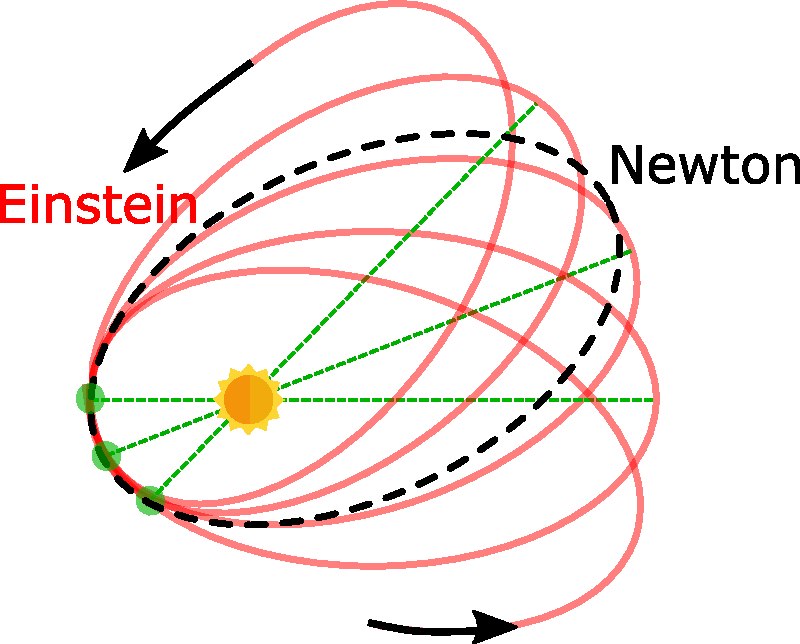
\includegraphics[width=0.82\linewidth]{../figs/pdf/en/fig-02-01.pdf}

% DOCX paragraph 173
\caption{\emph{Ilustración esquemática de la órbita de Mercurio. De acuerdo con la
teoría de la gravitación de Newton, debería ser cerrada (elipse de línea discontinua),
mientras que la teoría de la gravedad de Einstein (línea continua) nos dice que
debe cambiar continuamente, con el perihelio}\index{perihelio} \emph{desplazándose
en cada período orbital.}}\label{fig:02-01}
\end{figure}

% DOCX paragraph 175
¡Pero las observaciones astronómicas nos dicen algo totalmente diferente! Incluso
después de considerar las variaciones de la órbita debidas a otros cuerpos del
sistema solar, el perihelio\index{perihelio} de Mercurio varía más de lo que
predijo Newton: 0,1035 segundos de arco, o arcosegundos, en cada período orbital,
lo que corresponde a 0,4297 arcosegundos por
año.\textsuperscript{\hyperlink{note:02-02}{2}}

% DOCX paragraph 176
Durante décadas hubo intentos de explicar esta extraña anomalía del movimiento
de Mercurio de manera que fuera compatible con la teoría de la gravitación de
Newton. Y lo que tal vez sea aún más sorprendente ---y nos dará la oportunidad
de hacer un comentario importante al final del capítulo--- es que los astrónomos
de la época consiguieron reconciliar lo irreconciliable: ¡explicar el movimiento
anómalo de Mercurio mediante la ley de la gravitación de Newton! Sin embargo,
el precio que hubo que pagar, y que fue aumentando con el tiempo, fue postular
la presencia de un objeto celeste de masa y órbita muy precisas, por ejemplo
un planeta muy pequeño, cuya presencia influyera en la órbita de Mercurio y
generara, en el momento apropiado, la desviación observada.

% DOCX paragraph 177
El único problema de esa hipótesis, que por sí misma no estaba demasiado traída
por los pelos, era que el «planeta» tenía que ser prácticamente invisible:
tan pequeño que fuera imposible detectarlo con los telescopios de la época.

% DOCX paragraph 178
La hipótesis planteada para salvar la teoría de la gravedad de Newton representaba
una explicación \emph{plausible} ---al fin y al cabo, utilizaba una teoría de la
gravedad que se sabía que funcionaba bien---, pero al mismo tiempo \emph{improbable}:
requería la presencia artificial de un objeto perturbador nunca antes observado.
Bastaría recurrir al principio de la \emph{navaja de Occam}, que recibe su nombre
del filósofo y fraile franciscano inglés Guillermo de Ockham (1288-1347), para
considerar esta solución poco razonable. Así, cuando varias hipótesis son igualmente
plausibles para explicar un determinado comportamiento físico, la lógica férrea
de la navaja de Occam exige que se considere correcta la más simple. Obviamente,
la naturaleza no siempre elige la ruta más sencilla, de manera que la navaja de
Occam sirve, sobre todo, para descartar las hipótesis más engorrosas. Sin embargo,
la navaja de Occam nunca se llegó a utilizar con la órbita de Mercurio. Al contrario,
ante la ausencia de una teoría de la gravedad mejor y dado el respeto que se le
tenía a la teoría de Newton, la hipótesis del «pequeño planeta» podía satisfacer
a casi todo el mundo.

% DOCX paragraph 181
\section{Albert Einstein: una visión revolucionaria}\label{sec:02-einstein}

% DOCX paragraph 183
Más de dos siglos después de la publicación de los \emph{Principia} de Newton,
se ofreció al mundo una nueva teoría de la gravedad. No solo era aún más general
y proporcionaba una explicación natural del movimiento de Mercurio, sino que sus
predicciones sobre la precesión del perihelio\index{perihelio} coincidían
perfectamente con las observaciones. Esta teoría, que al principio resultó
incomprensible incluso para los científicos más ilustres de la época, hizo añicos
las profundas certezas sobre la gravedad adquiridas con Newton y propuso una
visión radicalmente distinta. Tan distinta que incluso hoy nos cuesta aceptar
sus implicaciones. Me refiero a la relatividad general: un resultado prodigioso
nacido de la mente de Albert Einstein (1879-1955).

% DOCX paragraph 184
La relatividad general\index{relatividad general} representa con razón una de
las teorías científicas más importantes jamás formuladas y es uno de los pilares
de la física moderna. Sin ella, la mayoría de las observaciones de física de
partículas, astrofísica y cosmología serían inexplicables.

% DOCX paragraph 185
Publicada a finales de 1915, a lo largo de los últimos cien años la relatividad
general\index{relatividad general} ha salido airosa de una larga serie de pruebas
experimentales, y actualmente es la teoría de la gravitación que mejor concuerda
con las observaciones astronómicas y los experimentos de laboratorio. Por otra
parte, representa un éxito aún más impresionante si consideramos que sigue siendo
una de las teorías matemáticamente más complejas jamás formuladas en física.
Resolver sus ecuaciones todavía constituye un desafío.

% DOCX paragraph 186
Pero aún es pronto para entrar en los detalles de esta teoría: lo haremos en el
próximo capítulo, donde llegaremos a comprender la importancia y el alcance
de sus implicaciones.

% DOCX paragraph 187
Mientras tanto, volvamos al misterioso planeta fantasma que era necesario para
explicar la órbita de Mercurio dentro de la teoría de la gravitación de Newton.

% DOCX paragraph 188
Hemos visto que esta explicación era posible e incluso plausible, pero no probable.
Es justamente este hecho el que animó a las mentes más audaces a buscar soluciones
menos engorrosas. Desde este punto de vista, la evolución de la teoría de la gravedad
---desde Galileo a Newton y luego a Einstein--- ilustra muy bien un punto fundamental:
es esencial ver una teoría científica como un marco lógico y matemático construido
para explicar las leyes de la naturaleza bajo determinadas condiciones. Proporciona,
en un contexto histórico, una explicación satisfactoria de las leyes de la naturaleza.
Por esta razón, cada teoría es intrínsecamente mejorable a medida que avanza nuestro
conocimiento de la naturaleza, en particular mediante observaciones o experimentos
que ponen en cuestión nuestras suposiciones iniciales, o a medida que se perfecciona
nuestra capacidad matemática para tratar los aspectos más débiles de la teoría.

% DOCX paragraph 189
Así pues, los desarrollos históricos de la gravedad descritos en este capítulo
nos muestran que una teoría física, a diferencia de una teoría matemática basada
en postulados y lógica, es solamente una representación provisional de una compleja
manifestación de la naturaleza. Nace para ser mejorada continuamente, revisada o
abandonada del todo si no puede explicar alguna manifestación nueva e inesperada
de las leyes de la naturaleza. Este es el destino que le aguarda incluso a la
mejor teoría de la gravedad que conocemos, la relatividad general\index{relatividad general},
en cuya fachada, unos cien años después de su construcción, han empezado a aparecer
unas diminutas grietas.
